\documentclass[conference]{IEEEtran}
\IEEEoverridecommandlockouts
% The preceding line is only needed to identify funding in the first footnote. If that is unneeded, please comment it out.
\usepackage{cite}
\usepackage{amsmath,amssymb,amsfonts}
\usepackage{algorithmic}
\usepackage{graphicx}
\usepackage{textcomp}
\usepackage{xcolor}
\usepackage[german]{babel}
\usepackage{rotating}
\usepackage{multirow}
\usepackage{url}

\def\BibTeX{{\rm B\kern-.05em{\sc i\kern-.025em b}\kern-.08em
T\kern-.1667em\lower.7ex\hbox{E}\kern-.125emX}}
\begin{document}

\bibliographystyle{IEEEtran}
\graphicspath{imgs}
\raggedbottom
\title{Erkennung von Design Patterns durch Maschine Learning}

\author{\IEEEauthorblockN{1\textsuperscript{st} Mehmet Aslan}
    \IEEEauthorblockA{\textit{Fakultät für Informatik} \\
        \textit{Hochschule Rosenheim}\\
        Rosenheim, Deutschland \\
        mehmet.aslan@stud.th-rosenheim.de}}

\maketitle
\thispagestyle{plain}
\pagestyle{plain}

\begin{abstract}
    Diese Seminararbeit setzt sich den Fokus, wie mithilfe von Machine Learning das Problem der Erkennung von Design Patterns gelöst werden kann. Dabei wird definiert, was unter Design Patterns im Rahmen dieser Seminararbeit zu verstehen ist und welchen Mehrwert die automatisierte Erkennung von diesen mit sich bringt.
    Zudem werden Ansätze erläutert, die diese Problematik ohne Einsatz von Machine Learning lösen. Nach diesem werden die groben notwendigen Schritte vorgestellt, wie die Erkennung von Design Patterns durch maschinelles Lernen gelöst werden kann. Dabei werden Methoden vorgestellt, die sich mit dieser Thematik befassen und wie diese Maschine Learning inkludiert haben.
\end{abstract}

\begin{IEEEkeywords}
    Machine Learning, Design Pattern Detection
\end{IEEEkeywords}

\section{Einleitung}
In der Entwicklung von Software-Systemen werden im Öfteren auf Probleme gestoßen, die bereits in der gleichen oder in ähnlicher Form bereits gelöst wurden. Für diese gängigen Probleme haben sich im Gegenzug gängige Lösungsblaupausen etabliert, womit sich diese lösen lassen. Diese sind in der Software-Entwicklung als Design Patterns bekannt.
Bei komplexen Software-Systemen ist das Nutzen dieser keine Seltenheit.
Dadurch, dass Software-Systeme durch neue oder angepasster Änderungen sich inkrementell weiterentwickeln, ist die strukturelle Verbesserung und Neugestaltung des unterliegenden Quellcodes ohne Veränderung des Programmverhaltens, auch Code-Refactoring genannt, Teil des Entwicklungsprozesses.
Bei Code-Refactoring muss man den gewissen Systemkontext während des Prozesses im Kopf beibehalten, um den betrachte Programmfluss im Quellcode zu verstehen.
Dabei können Programmstrukturen über mehreren Quellcode-Dateien, Module oder Bibliotheken verteilt sein. Deshalb kann der Erhalt des Systemkontextes im Verständnis schwerfallen, vor allem bei Design Patterns. Um dagegenzuwirken, kann eine werkzeug-gestützte Hilfestellung mithilfe von Machine Learning den Refactoring-Prozess mit Umgang von Design Patterns einfacher gestalten.
Im Rahmen dieser Problematik setzt sich diese Seminararbeit die Untersuchung der Erkennung von Design Patterns mit Machine Learning als Fokus. Dabei ist die Arbeit in folgende Segmente untergliedert: gesetzte Einschränkung für die Untersuchung, Ansätze aus nicht Machine Learning Gebieten und die notwendigen Schritte für die Erstellung eines Modells sowie zweier Methoden, die die Maschine Learning bei der Erkennung inkludieren.


\section{Eingrenzungen der Seminararbeit}
Um mit der Erkennung der Design Patterns anzufangen, muss vorerst definiert werden, welche Design Patterns überhaupt zu betrachten sind. Da der Fokus dieser Seminararbeit auf der Analyse von Quellcode liegt, werden hier deren Einsatz in Programmiersprachen betrachtet.
Das Werk, womit der Begriff der Design Patterns in den Köpfen den Software-Entwicklern am ehesten assoziieren, sind die Konstrukte, die im Werk "Design Patterns: Elements of Reuseable Software" definiert \cite{gamma1994design} sind. Diese Design Patterns sind ebenfalls unter dem Begriff `GoF Design Patterns' bekannt. Da der Fokus in diesem Werk den Einsatz von Design Patterns in einem
objektorientierten Kontext betrachtet werden, wird diese auch so im weiteren Verlauf der Untersuchung übernommen. Obwohl die Erläuterungen der GoF Design Patterns ursprünglich in der Programmiersprache C++ verfasst wurden, wird in dieser Arbeit deren Einsatz ebenfalls in der objektorientierten Programmiersprachen Java betrachtet.
Dabei werden die Design Pattern in folgende Kategorien unterteilt werden \cite[p. 5797]{Yarahmadi2020}

\begin{figure}[h]
    \centering
    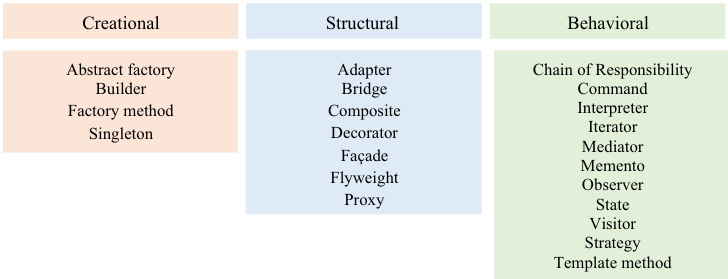
\includegraphics[width=\linewidth]{imgs/gof.png}
    \caption{Design Pattern Kategorien nach GoF}
\end{figure}


\newpage

\section{Alternative Ansätze}

Neben den Lösungsansätzen aus dem Machine Learning Bereich, wurden Verfahren aus anderen Bereichen der Informatik eingesetzt, um die Erkennung von Design Patterns bis zu einem gewissen Grad zu automatisieren.
In diesem Abschnitt der Seminararbeit werden einige Ansätze vorgestellt.

\subsection{Graphenanalyse}

In den meisten Verfahren ist der Quellcode in seiner ursprünglichen Form als rohe Textdatei als Eingabe nicht geeignet, um mit einer hohen Genauigkeit Design Patterns zu erkennen.
Aus diesem Grund ist daher notwendig, dass man die Quelldateien in eine andere Form transformiert, um mit diesen besser arbeiten zu können. Deshalb ist die Transformation der Quelldateien in eine graphenbasierte Form ein bereits etablierter Ansatz.
Durch den Einsatz von Knoten, Kanten und Subgraphen können die Beziehung und Zusammensetzung der einzelnen Komponenten in den Quelldateien in einer Programmiersprachen-agnostischen Form repräsentiert werden.
Dabei dienen Eigenschaften von Graphen und graphenbasierte Algorithmen wichtige Werkzeuge in diesen Ansätzen. Beispielsweise wird in der Arbeit von Pradhan et al. \cite{PradGraph} die Eigenschaften der Graphenisomorphie, um aus dem Quellcode-Graphen Design Patterns zu erkennen.
Dabei ist das zu suchende Design Pattern als Subgraph Teil des Quellcode-Graphen. Im Quellcode-Grahen wird mithilfe eines bereits definierten Graphen, was ein Design Pattern darstellt, nach isomorphen Teilgraphen im Quellcode-Graphen gesucht.
Zusätzlich wird die normalisierte Kreuzkorrelation genutzt, um die Ähnlichkeit zwischen den gefundenen Teilgrafen und dem gesuchten Design Pattern zu quantifizieren.
Ein weiteres Beispiel wäre der Ansatz von Bernardi et al., die eine domänenspezifische Sprache entwickelt, womit Design Patterns als ein Set von Regeln definiert werden kann \cite{Bernardi2013AMG}, die auf einen Quellcode-Graphen angewendet werden können. Diese Regeln werden dann genutzt, um Design Patterns im Quellcode-Graphen zu erkennen.

\subsection{Analyse durch Software-Metriken}

Um gestützte Aussagen über Software-System zu tätigen, werden in der Software-Entwicklung Metriken eingesetzt, um Eigenschaften wie Größe, Komplexität, Kopplug usw. des betrachteten Software-Systems zu quantifizieren.
Dadruch erschließt sich die Möglichkeit, Hypothesen über das Software-System zu tätigen. Diese Metriken können bei der Erkennung von Design Patterns als Ansatz genutzt werden, um Anzeichen oder Muster in einem Software-System zu erkennen.
In ihrer Arbeit schlagen Issaoui et al. \cite{Issaoui2015} einen Prozess vor, wie mithilfe von Software-Metriken der Suchraum für Design Patterns eingeschränkt werden kann. Dabei werden konkrete Eigenschaften und Metrikwerte bestimmt, die das jeweilige Design Pattern kennzeichnen.
Das Gesamte zu betrachtende Software-System wird durch die vorher definierten Metriken quantifiziert und es werden diejenigen Komponenten des Software-Systems weiter betrachtet, die die vorher festgelegte Einschränkungen erfüllen.
Dieser Ansatz dient als ergänzende Methodik für existierende Prozesse, um die Menge möglicher Kandidaten zu reduzieren.
Ashish et al. hingegen nutzen Software-Metriken, um ein Dataset zu generieren, die Design Patterns verschiedene Software-Metriken und Werte zu ordnen \cite{Ashish2016}. Dabei dient dieses Dataset als Eingabe für Data Mining- und maschinelle Lernalalgorithmen, um Relationen zwischen Software-Metriken und Design Patterns abzuleiten.


\subsection{Analyse durch Anfragen}

Dieser Ansatz orientiert sich an relationale Datenbanken. Dabei wird an ein Set von Daten eine Anfrage gestellt und als Ergebnis wird ein Subset der Daten zurückgegeben, die die Bedingungen der gestellten Anfrage erfüllen. Dieses Konzept lässt sich auf Quellcode ebenfalls anwenden.
Jedoch muss der Quellcode in eine Form transformiert, an diesem die Anfragen durchgeführt werden können. Dazu eigenen sich baumartige Formate wie Abstract Syntax Trees (AST) oder Extended Markup Language (XML) Dokumente.
ASTs werden bei dem Compile-Vorgang verwendet, um die Struktur des jeweiligen Quellcodes zu repräsentieren. XML-Dokumente erfüllen einen ähnlichen Zweck wie AST in diesem Kontext,
bieten zusätzlich die Möglichkeit an, durch Einsatz von Attributen zusätzliche Metainformationen an die Knoten mitzugeben. Diese Strukturen ermöglichen das Traversieren der jeweiligen Struktur durch Angabe von der zu begehenden Pfade in Form von Anfragen.
Den gesuchten Design Patterns werden in Form dieser Anfragen abgelegt und durch an der jeweiligen Baumstruktur durchgeführt.
Bouassida und Ben-Abdallah stellen einen Prozess wie mithilfe von Information-Retrieval-Techniken, Artefakte des Quellcodes wie Klassen, Methoden oder Beziehungen zwischen Entitäten als XML-Dokument zu repräsentieren \cite{bouassida2010pattern}.
Mit Anfragen können nun in diesem nach Design Patterns oder nach "spoiled patterns", abgewandelten Design Patterns, gesucht werden.


\newpage

\section{Machine Learning Ansatz: Grober Ablauf}

Das Erscheinen von kostenlosen Open-Source-Projekten wie TensorFlow, sklearn oder PyTorch sorgte dafür, dass im Verlauf der Jahre der Zugang und die Einstiegshürde geringer wurde, sodass der Einsatz von Machine Learning
weiter zunahm. Machine Learning Algorithmen sind unter anderem dafür geeignet, um Eingaben zu klassifizieren, neue synthetische Daten zu generieren oder eine Regressionsanalyse durchzuführen. Im Feld der Design Pattern Erkennung wurden Machine Learning basierende Ansätze als Kern des Erkennungsprozesses oder als ergänzender Schritt im Prozess verwendet. Dadurch erlangte Machine Learning immer weiter Popularität \cite[p. 5805]{Yarahmadi2020}.
In diesem Abschnitt der Seminararbeit werden grob die notwendigen Schritte vorgestellt, wie theoretisch solch ein Prozess mit Machine Learning im Kern aussehen kann.

\subsection{Data Gathering}
In dem initialen Zustand ist ein untrainiertes Machine Learning Modell blank. In dieser Situation ist Modell nicht in der Lage, die erwarteten Anforderungen zu erfüllen, da das Modell kein Wissen über die Eingaben besitzt. Aus diesem Grund muss notwendige Wissen dem Modell beigebracht werden.
Data Gathering beschreibt im Machine Learning Prozess, wie die Rohdaten zu einem Kollektiv zusammengetragen, die im weiteren Verlauf der Seminararbeit als Dataset betrachtet wird. Dabei sollte beachtet werden, dass es sich hierbei um Rohdaten handelt. Die Daten werden in deren darauf folgenden Schritten weiter bearbeitet.
Für die Erstellung des Datasets eignen im Kontext der Design Pattern Erkennung für Machine Learning vor allem Open-Source-Projekte. Viele der Prozesse nutzen Quelldateien als unverarbeitete Eingabe \cite[p. 5801]{Yarahmadi2020}, die in den darauffolgenden Phasen um Informationen ergänzt oder transformiert werden. Open-Source-Projekte eignen sich hierfür, da die Lizenzen für diese meistens das freie Weiternutzen der Quelldateien erlauben.
Folgende Open-Source werden am häufigsten verwendet \cite[p. 5817]{Yarahmadi2020}:

\begin{itemize}
    \item JUnit
    \item JHotDraw
    \item JRefactory
    \item Java AWT
\end{itemize}

\subsection{Explorativ Data Analysis}

Explorativ Data Analysis (EDA) beschäftigt sich mit der Analyse des Datasets, um Muster, Trends, Abweichungen oder andere relevante Informationen im Dataset zu identifizieren \cite{IBM}.
Das Hauptziel von EDA besteht darin, ein besseres und tieferes Verständnis für das Dataset zu gewinnen, bevor das Dataset weiter verarbeitet wird. Dabei werden verschiedene Methoden und Techniken verwendet,
um die Daten zu visualisieren, Beziehungen zwischen Eingabeparametern und statistische Analysen durchzuführen. Je nach Dataset können bereits hier wie Data Cleaning oder Feature Extraction, die auf diesen Schritt folgen, bereits hier durchgeführt werden.
Dabei können je nach Verfügbarkeit des Datasets folgende Methoden und Techniken hilfreich sein:

\begin{itemize}
    \item \textbf{Data Visualization}: Durch Einsatz von Diagrammen, Plots oder Histogrammen können Muster, Trends oder Ausreißer im Dataset erkannt werden.
    \item \textbf{Statiscal Analysis}: Methoden wie Mittelwerte, Varianzen, Korrelationen oder Clusteranalysen können statistische Zusammenhänge bereits im Vorfeld erkannt werden.
\end{itemize}


\subsection{Data Preprocessing}

Data Preprocessing beschreibt den notwendigen Schritt, um die Rohdaten in eine Form zu bringen, mit denen das Machine Learning Modells umgehen kann.
Dieser Schritt beinhaltet unter anderem die Bereinigung, Transformation und Formatierung der Rohdaten. Dadurch kann die Leistungsfähigkeit des ausgewählten Modells verbessert werden.
Im Kontext der Design Pattern Erkennung können folgende Schritte von Bedeutung sein \cite{Anunaya_2023}:

\begin{itemize}
    \item \textbf{Data Cleaning}: Hier werden unerwünschte Daten oder fehlerhafte Daten aus dem Dataset entfernt oder korrigiert. Dies kann das Entfernen von Duplikaten, das Behandeln fehlender Werte oder das Korrigieren von inkonsistenten oder fehlerhaften Daten inkludieren.
    \item \textbf{Tokenization}: Der Quellcode wird in kleinere Einheiten, die auch Tokens genannt werden, aufgeteilt. Tokens können Wörter, Zeichen oder andere diskrete Information sein, die Informationen darstellen
    \item \textbf{Normalization}: Bei Machine Learning Modelle kann die statistische Verteilung der Eingabewerte die Leistung des Modells teils mehr, teils weniger beeinflussen. Daher kann die Normalisierung der Eingangsdaten durch Min-Max Scaling, Standard-Scaling oder Techniken ausschlaggebend für die Leistung des Modells sein.
    \item \textbf{Data Formatting}: Die Daten im Datenset werden in eine Form transformiert, mit denen das Machine Learning Modell umgehen kann. Unter anderem können die Dateien in Vektoren, Matrizen oder in andere Datenstrukturen umgewandelt werden.
\end{itemize}

\newpage

\subsection{Feature Extraction}

Bei der Design Pattern Erkennung durch Machine Learning bezieht sich Feature Extraction auf den Prozess der Extraktion relevanter Merkmale oder Eigenschaften aus den Rohdaten, um das Machine Learning Modell zu trainieren.
Diese extrahierten Merkmale dienen als Eingabe für das Modell, um Design Patterns zu identifizieren. Die Auswahl dieser Merkmale erfolgt in der Regel basierend auf das Fachwissen, Erfahrung und dem verfügbaren Dataset.
Aus diesem Grund existieren keine definitiven Merkmale für diese Problemstellung. Jedoch können nach Verfügbarkeit folgende Merkmale bei der Design Pattern Erkennung relevant sein:

\begin{itemize}
    \item \textbf{Strukturelle Merkmale}: Bei der Analyse von Quellcode können Informationen über Klassen, Beziehungen, Vererbungen und anderer strukturellen Elemente enthalten. Diese Merkmale könnten Auskunft über Hierarchie, Abhängigkeiten und Interaktionen zwischen Klassen anbieten und zur Erkennung von Design Patterns beitragen.
    \item \textbf{Textuelle Merkmale}: Textbasierte Information wie Kommentare, Bezeichner oder andere Textelemente im Quellcode können ebenfalls als Merkmale betrachtet werden. Diese könnten Benennungskonventionen, bestimmte Ausdrücke oder Schlüsselwörter enthalten, die charakteristisch zu einem bestimmten Design Pattern zugeordnet werden können.
    \item \textbf{Metrikenbasierte Merkmale}: Software-Metriken können genutzt werden, um Eigenschaften wie Komplexität, Kopplung oder Kohäsion in einem Software-System zu quantifizieren und das Dataset mit diesen zu ergänzen. Diese können genutzt werden, um mögliche Kandidaten zu identifizieren.
    \item \textbf{Verhaltensbasierte Merkmale}: Bei vorhandenem Quellcode können das Ausführungsverhalten des Software-Systems auch als relevante Merkmale betrachtet werden. Dies inkludiert unter anderem das Aufzeichnen von Methodenaufrufen oder die Analyse von Ausführungszeiten beinhalten.
\end{itemize}


\subsection{Model Selection}

Bei der Erkennung von Design Patterns handelt es sich um ein Klassifizierungsproblem. Bei der Eingabe der Eingangsparameter werden durch das Machine Learning Modell mögliche Klassen mit gewissen Wahrscheinlichkeiten zuzuordnen.
Da das Resultat der Berechnung des Modells relevant ist und einer Eingabe eine oder mehrere Klassen zugeordnet werden können, kann man die Menge der möglichen Modelle auf die eingrenzen, die zum Bereich des Supervised Learnings zugeordnet werden können.
Bei Supervised Learning versucht das Machine Learning Modell eine Funktion zu approximieren, die die Eingabeparameter auf eine oder mehrere Klassen abbildet. Dies dient auch zur Klassifizierung von neuen und unbekannten Daten.
Je nach Dataset können folgende Auswahl an Modelle verwendet werden:

\begin{itemize}
    \item \textbf{Random Forest}: Random Forest Modelle ist ein sogenanntes Ensemble-Modell, die intern aus mehreren Decision Trees besteht, deren Ausgabe zu einem Resultat zusammengefasst wird. Decision Trees verwenden angelernte Entscheidungsregeln, um der Eingabe mehrere Klassen zuzuordnen \cite{scikit_random_forest}.
    \item \textbf{Support Vector Machine}: Support Vector Machines versuchen, zwischen den Eingaben eine oder mehrere Trennflächen (auch Hyperplanes genannt) zu definieren, die die Klassen voneinander trennen \cite{scikit_svm}.
    \item \textbf{Neuronal Networks}: Neuronal Networks wie Convolutional Neural Networks (CNNs) oder Recurrent Neural Networks (RNNs) eignen sich als effektive Modelle bei der Erkennung von Design Patterns im Quellcode. CNNs sind passend, um visuelle Muster in Quellcode zu erkennen, während RNNs die Sequenzstruktur von Quellcode analysieren können \cite{scikit_nn}.
    \item \textbf{Multiclass Logistic Regression}: Bei Multiclass Logistic Regression wird für jede Design Pattern-Klasse eine separate binäre logistische Regression durchgeführt. Die Wahrscheinlichkeiten der einzelnen Klassen werden berechnet und das Modell trifft eine Entscheidung, indem es die Klasse mit der höchsten Wahrscheinlichkeit auswählt \cite{scikit_lm}.
    \item \textbf{Naive Bayes}: Naive Bayes ist ein probabilistisches Modell, das auf dem Bayes-Theorem basiert. Es kann für die Klassifikation mit mehreren Klassen verwendet werden, indem es die Wahrscheinlichkeiten der einzelnen Design Pattern-Klassen basierend auf den Merkmalen berechnet \cite{scikit_bayes}.
\end{itemize}

\newpage

\subsection{Model Training}

Nach der Auswahl des Modells kann die eigentliche Trainingsphase des Machine Learning Modells gestartet werden.
Zuerst muss das Modell initialisiert werden. Je nach Modell können bei der Initialisierung zusätzliche Parameter erforderlich sein, die die Struktur oder das Verhalten des Modells beeinflussen. Diese Parameter werden auch Hyperparameter genannt und werden von dem Anwender unabhängig von dem Dataset festgelegt.
Nachdem das Dataset sich in einer Form befindet, mit der das Modell umgehen kann, wird meistens das vorhandene Dataset in zwei gespalten: in ein Training Dataset und ein Validation Dataset.
Das Training Dataset wird verwendet, um das Modell trainieren, während das Validation bei der Evaluation des Modells verwendet wird. Die Aufteilung verläuft im Schnitt so ab, dass ungefähr mehr als die Hälfte der Einträge im Dataset dem Training Dataset und der Rest den Validation Dataset zugeordnet werden.
Die Dauer des Trainings hängt von dem Umfang des Dataset, der Rechenleistung der Host-Maschine und der Komplexität des Machine Learning Modells ab.

\subsection{Model Evaluation}

Nachdem das Training des Modells abgeschlossen wurde, steht die Evaluation des Modells an.
Dazu wird das Validation Dataset dem Modell zur Klassifizierung übergeben und betrachtet, wie die Ergebnisse der Berechnung des Machine Learning Modells von der eigentlichen Klassifizierung abweichen.
Um diese Abweichung zu quantifizieren, können folgende Auswahl an Metriken verwendet werden:

\begin{itemize}
    \item \textbf{Accuracy}: Die Genauigkeit ist ein Maß zwischen 0 und 1 und gibt an, wie gut das Modell insgesamt in der Lage ist, korrekte Vorhersagen zu treffen. Sie gibt den Anteil der korrekten Vorhersagen zur Gesamtzahl der Vorhersagen an. Je näher das Ergebnis bei 1, desto besser die Vorhersage der Klassen \cite{scikit_accuracy}.
    \item \textbf{Precision \& Recall}: Präzision und Recall sind Metriken, die insbesondere für unbalancierte Klassenverteilungen relevant sind. Die Präzision gibt den Anteil der korrekt als positiv vorhergesagten Instanzen zur Gesamtzahl der als positiv vorhergesagten Instanzen an \cite{scikit_pre}. Der Recall gibt den Anteil der korrekt als positiv vorhergesagten Instanzen zur Gesamtzahl der tatsächlich positiven Instanzen an \cite{scikit_recall}.
          Ein hoher Präzisionswert zeigt an, dass das Modell in der Lage ist, die relevanten Muster genau zu erkennen. Ein hoher Recall zeigt an, dass das Modell in der Lage ist, die meisten tatsächlich positiven Instanzen zu erfassen.
    \item \textbf{F1-Score}: Der F1-Score ist eine kombinierte Metrik, die Präzision und Recall berücksichtigt. Er gibt das harmonische Mittel zwischen Präzision und Recall an \cite{scikit_f1}. Ein hoher F1-Score zeigt an, dass das Modell sowohl eine hohe Präzision als auch einen hohen Recall aufweist.
    \item \textbf{Confusion Matrix}: Die Konfusionsmatrix ist eine Tabelle, die die Anzahl der richtigen und falschen Vorhersagen für jede Klasse darstellt \cite{scikit_conf}. Sie gibt detaillierte Informationen über die Leistung des Modells für jede Klasse und ermöglicht das Berechnen von verschiedenen Metriken wie Genauigkeit, Präzision und Recall für jede Klasse.
    \item \textbf{ROC-Curve \& AUC}: Die ROC-Curve (Receiver Operating Characteristic) und der AUC-Wert (Area Under the Curve) sind Metriken, die die Leistung eines Modells bei der Klassifikation von Daten über verschiedene Schwellenwerte hinweg bewerten \cite{scikit_roc}. Sie sind insbesondere relevant, wenn die Trade-offs zwischen True Positive Rate (TPF; auch Recall gennant) und False Positive Rate (FPR) betrachtet werden sollen.
          Eine perfekte Klassifikation würde zu einer ROC-Curve führen, die den Punkt (0,1) erreicht, was bedeutet, dass die TPR 100 \% und die FPR 0 \% beträgt. Ein zufälliges Klassifikationsmodell würde eine ROC-Curve erzeugen, die der diagonalen Linie entspricht. Der AUC-Wert gibt den Bereich unter der ROC-Curve an und dient als Zusammenfassung der gesamten Leistung des Modells. Ein AUC-Wert von 1 bedeutet, dass das Modell eine perfekte Trennung zwischen den Klassen erreicht, während ein AUC-Wert von 0.5 darauf hinweist, dass das Modell nicht besser ist als eine zufällige Klassifikation.
\end{itemize}

\newpage

\subsection{Hyperparameter-Tuning}

Falls durch die Evaluation des Modells festgestellt wird, dass die Leistungsfähigkeit des Modells nicht den Erwartungen entspricht, kann man durch Erweiterung des Datasets oder durch Hyperparameter-Tuning versuchen, dessen Leistung zu verbessern.
Dadurch, dass die Hyperparameter des Machine Learning Modells unabhängig von des Dataset gesetzt werden, gibt es keine analytische Methode, um die Hyperparameter für jeden Anwendungsfall zu optimieren. Aus diesem Grund ist die Optimierung der Hypterparameter eher ein Trail \& Error-Verfahren.
Im Allgemeinem kann das Hyperparameter-Tuning in folgende Schritte untergliedert werden:
\begin{enumerate}
    \item \textbf{Auswahl Hyperparameter}: Die Auswahl der betrachtenden Hyperparameter ist abhängig von dem jeweiligen Machine Learning Modell.
    \item \textbf{Definition des Suchraums}: Den ausgewählten Hyperparameter wird entweder ein Wertebereich oder einem diskrete Werte zugeordnet.
    \item \textbf{Auswahl der Tuning-Methode}: Folgende Tuning-Methoden werden am häufigsten verwendet
          \begin{itemize}
              \item Random Search: Random Search probiert verschiedene Kombinationen von Hyperparametern aus, wobei jeder Hyperparameter aus einem vordefinierten Wertebereich oder einer Verteilung gezogen wird. Diese Methode hilfreich, um den Suchraum einzugrenzen und mit Grid Search die optimale Parameterkombination zu determinieren \cite{scikit_random}.
              \item Grid Search: Grid Search sucht nach allen mölglichen Kombination der Hyperparameter traniert und evaliuiert. Diese kann nach der Menge der möglichen Operationen recheninteniv und dementsprechend lang dauern. Zuerst sollte ein Random Search durchgeführt werden, um den Suchraum zu verkleinern \cite{scikit_grid}.
          \end{itemize}
    \item \textbf{Festlegen der Evaluierungsmetrik}: Diese Metrik wird genutzt, um die Leistung von der Tuning-Methode determinierte Iteration des Modells zu bewerten. Hierzu kann einer der vorher erwähnten Metriken genutzt werden.
    \item \textbf{Durchführen des Tuning-Verfahren}: Die ausgewählte Tuning-Methode kann nun gestartet werden. Das Training und die Evaluation sind meistens darin enthalten.
    \item \textbf{Manuelle Validierung und Test}: Um sicherzustellen, dass das Modell gut generalisiert ist, sollte die durch die Tuning-Methode bestimmte Hyperparameter-Kombination mit einem separaten Training und Validation Dataset überprüft werden.
\end{enumerate}

\newpage

\section{Vorstellung von Machine Learning Ansätzen}

\subsection{Design Pattern Detection mit Metriken als Input}

Uchiyama et al. nutzen in ihrem Lösungsvorschlag nicht eine Repräsentation des Quellcodes als Eingabe für ihr Machine Learning Modell, sondern nutzen von dem Quellcode abgeleitete Metriken als Eingabe\cite{dodmetrics}.
Dabei kann die von ihnen vorgeschlagene Prozess in folgende Schritte unterteilt werden:


\subsubsection*{P1. Define Patterns}
In diesem Prozess wurde auf die 23 GoF Design Patterns zurückgegriffen. Aus den drei Kategorien wurde sich für `Adapter'-, `Singelton'- `Template Method'-, `State'- und `Strategy'-Patterns als zu erkennende Design Patterns entschieden, sodass jede Kategorie von den GoF Patterns mindestens einen Vertreter hat. Rollen sind hier Mikrostrukturen, in Teil der Struktur der Design Patterns ist. Dieser Prozess berücksichtigt diese fünf Patterns und die 12 abgeleiteten Rollen \cite[p. 4]{dodmetrics}.

\subsubsection*{P2. Decide Metrics}
Um diese Metriken abzuleiten, wurde hier das Goal Question Metric (GQM)-Methode angewendet. In der GQM werden Ziele als Goals definiert, die weiter in Fragen (Questions) aufgeteilt werden, sodass durch Beantwortung dieser Fragen bestimmt werden kann, ob das gesetzte Ziel erreicht wurde oder nicht. Für die Beantwortung dieser Fragen werden Metriken (Metrics) abgeleitet. Anhand dieser Methode für jedes zu identifizierende Design Pattern ein Set an Metriken definiert.
Folgende Metriken sind das Resultat \cite[p. 7]{dodmetrics}:

\begin{table}[h!]
    \begin{tabular}{ |c|c| }
        \hline
        Abbreviation & Content                                        \\
        \hline
        NOF          & Number of fields                               \\
        \hline
        NSF          & Number of static fields                        \\
        \hline
        NOM          & Number of methods                              \\
        \hline
        NSM          & Number of static methods                       \\
        \hline
        NOI          & Number of interfaces                           \\
        \hline
        NOAM         & Number of abstract methods                     \\
        \hline
        NORM         & Number of overridden methods                   \\
        \hline
        NOPC         & Number of private constructors                 \\
        \hline
        NOOF         & Number of object fields                        \\
        \hline
        NCOF         & Number of other classes with field of own type \\
        \hline
        NMGI         & Number of methods generating instances         \\
        \hline
    \end{tabular}
    \caption{Ausgewählte Metriken}
    \label{tabel:1}
\end{table}


\subsubsection*{P3. Maschine Learning}

Als Machine Learning Modell wird in dieser Methodik ein neuronales Netz verwendet \cite[p. 5]{dodmetrics}. Dieser besteht aus einem Input-Layer, was die Metriken als Eingabe entgegennimmt, einem Output-Layer für die Ausgabe der Resultate und einer Anzahl von Hidden-Layern zwischen dem Input- und Output-Layer.
Die Länge des Input-Layers entspricht der Länge Eingangsvektors. Diese ist bestimmt durch die Anzahl der zu verarbeitenden Metriken. Die Länge des Output-Layers entspricht der Anzahl der möglichen Rollen.
Die Anzahl der Hidden-Layer entspricht der Länge des Input-Layers. Als Transferfunktion wird hier die Sigmoid-Funktion verwendet.
Um das Modell zu optimieren, wird bei neuronalen Netzwerke bekannte Back-Propagation verwendet, um die Anzahl an falschen Klassifizierungen zu vermeiden.

\subsubsection*{P4. Candidate Role Judgment}

Der Quellcode wird durch die vorgestellten Metriken in Tabelle \ref*{tabel:1} quantifiziert und als Eingabe in das Machine Learning Modell übergeben. Das Modell weist als Ergebnis der Klassifizierung für alle zu beurteilenden Rollen Werte zwischen 0 und 1 zu. Je größer dieser Wert, desto wahrscheinlicher die korrekte Rollenzuweisung.
Um die Ausgabewerte zu normalisieren und vergleichbar zu machen, werden sie skaliert, sodass ihre Summe 1 ergibt \cite[p. 5]{dodmetrics}. Diese Normalisierung ermöglicht die Verwendung eines gemeinsamen Schwellenwerts für den Vergleich. Die normalisierten Ausgabewerte werden als "Role Agreement Valle" bezeichnet, wobei ein höherer Wert auf eine höhere Wahrscheinlichkeit hinweist, dass die Rolle korrekt ist.
Der Schwellenwert zur Bestimmung der Rollen wird als Kehrwert der Anzahl der zu erkennenden Rollen festgelegt. In diesem Fall beträgt der Schwellenwert 1/12 (d.h. 0.0834), da derzeit 12 Rollen berücksichtigt werden.

\subsubsection*{P5. Pattern Detection}

Das Machine Learning ist in der Lage, einzelne Rollen in den Design Patterns zu erkennen, jedoch ist nicht in der Lage, eine Aussage über Relation der Rollen zu tätigen. Um darüber Aussagen treffen zu können, wird ein ergänzender Schritt eingeführt. In diesem werden nacheinander alle Kombinationen von Rollen, die mit der Struktur der Design Patterns übereinstimmen, betrachtet und überprüft, ob die Beziehungsrichtungen zwischen den Rollen mit der Design Pattern Struktur übereinstimmen.
Wenn die Beziehungsrichtungen und Rollen übereinstimmen, wird das Design Pattern erkannt. Derzeit behandelt diese Methode Vererbungs-, Schnittstellenimplementierungs- und Aggregationsbeziehungen. Um den Unterschied zwischen diesen Beziehungstypen zu verdeutlichen, wird der "Relation Agreement Value" eingeführt \cite[p. 6]{dodmetrics}, der diesen quantifiziert widerspiegelt. Der Relation Agreement Value ist 1.0, wenn der Typ und die Richtung der Zielbeziehung mit der Beziehung der Struktur des Design Pattern übereinstimmen, und 0.5, wenn nur die Richtung übereinstimmt. Wenn die Richtung nicht übereinstimmt, wird der Relation Agreement Value zu 0.
Der notwendigen Schritte zu Ermittelung dieses Wertes wird hier nicht weiter betrachtet.

\subsubsection*{Evaluation}

Das Verfahren wurde mit sowohl mit `kleinen' Applikationen (Mustercode aus Lehrbüchern) als auch mit `größeren' Applikation wie mit den Java-Frameworks JUnit, Spring Framework und der Java Standardbibliothek getestet \cite[p. 7]{dodmetrics}.
Aus den Testpool der kleinen Programme mit einem Umfang mit 60 Proben wurden 20 und bei den "größeren" Applikationen wurden von 158 möglichen Proben 126 zu der Evaluation verwendet.
Dabei wurden die Recall und Precision Metriken zu Qualifizierung dieser Methode genutzt und folgende Werte ermittelt \cite[p. 8]{dodmetrics}:

\begin{sidewaystable}
    \centering
    \caption{Precision und Recall für Design Pattern Erkennung}
    \label{table:2}
    \begin{tabular}{|c|c|c|c|c|c|c|}
        \hline
                        & \multicolumn{2}{|c|}{Number of test data} & \multicolumn{2}{|c|}{Precision (\%)} & \multicolumn{2}{|c|}{Recall (\%)}                                           \\
        \hline
        Pattern         & Small-scale                               & Large-Scale                          & Small-scale                       & Large-Scale & Small-scale & Large-Scale \\
        \hline
        Singelton       & 6                                         & 6                                    & 60                                & 46          & 100         & 83          \\
        \hline
        Template Method & 6                                         & 7                                    & 86                                & 67          & 100         & 57          \\
        \hline
        Adapter         & 4                                         & 7                                    & 100                               & 100         & 75          & 57          \\
        \hline
        State           & 2                                         & 6                                    & 50                                & 50          & 100         & 85          \\
        \hline
        Strategy        & 2                                         & 6                                    & 67                                & 50          & 100         & 100         \\
        \hline
    \end{tabular}
\end{sidewaystable}

Wie aus Tabelle \ref{table:2} zu entnehmen ist, liefert diese Methode für `kleinere' als auch `größere' Applikation hohe Precision- und Recall-Werte, was für eine gute Klasszifierungkapazität der Methode spricht.

Um die Leistung dieses Ansatzes zu vergleichen, wurde diese mit anderen Methoden verglichen, die ebenfalls zur Erkennung von Design Patterns entwickelt wurden.
Dabei wurde die Methoden von Tsantalis et al.(TSAN) \cite{4015512}, die auf Similarity Scoring beruht, und Dietrich and Elgars (DIET)\cite{DIETRICH2007108} zum Vergleich hergezogen. Diese Verfahren nutzen beide Java-Quellcode als Basis für die Eingabe und können Design Patterns erkennen, die auch in dieser Methodik feststellbar sind.
Das hier vorgestellte Verfahren wurden mit den Design Patterns getestet, die zum Vergleich hergezogenen Verfahren erkennbar sind. Zum Vergleich wurde der F1-Score ermittelt \cite[p. 9]{dodmetrics}:

\begin{table}[h]
    \centering
    \caption{Durchschnittlicher F1-Score (gegen TSAN)}
    \label{table:3}
    \begin{tabular}{|c|c|c|}
        \hline
                      & Small-scale programs & Large-scale programs \\
        \hline
        Diese Methode & 0.67                 & 0.56                 \\
        \hline
        TSAN          & 0.39                 & 0.36                 \\
        \hline
    \end{tabular}
\end{table}

\begin{table}[h]
    \centering
    \caption{Durchschnittlicher F1-Score (gegen DIET)}
    \label{table:4}
    \begin{tabular}{|c|c|c|}
        \hline
                      & Small-scale programs & Large-scale programs \\
        \hline
        Diese Methode & 0.69                 & 0.55                 \\
        \hline
        DIET          & 0.50                 & 0.35                 \\
        \hline
    \end{tabular}
\end{table}

Wie ist aus den Tabellen \ref{table:3} und \ref{table:4} zu entnehmen ist, erzielt dieses Modell im Durchschnitt bessere F1-Scores, was im Ganzen für eine bessere Leistung des hier vorgestellten Verfahrens spricht.

\newpage

\subsection{DPD \textsubscript{f}}

In ihrer Arbeit stellen Nazar et al. \cite{NAZAR2022111179} eine auf Feature basierende Methode zur Erkennung von GoF Design Patterns mit Machine Learning vor, die neben der Struktur auch lexikale Features als Eingabe entgegennimmt. Im weiteren Verlauf wird diese Methode als DPD\textsubscript{f} bezeichnet.
Die Methode kann in folgende Schritte untergliedert werden:

\subsubsection*{Data Collection}
Anstatt ein existierendes Dataset wie P-MARt\cite{pmart} zu nutzen, wurde dieses Dataset zum Benchmark genutzt und ein eigenes Dataset erstellt, das DPD\textsubscript{F}-Corpus benannt wurde \cite[p. 4]{NAZAR2022111179}.
Dieses besteht aus Java-Quelldateien, die von dem Github Java Corpus stammen, und im weiteren Verlauf bereinigt wurden.
Das Labeling wurde durch Crowdsourcing ermöglicht, indem das Werkzeug CodeLabeller genutzt wurde. Dabei wurde der DPD\textsubscript{F}-Corpus von Menschen mit Labeln versehen, die mindestens zwei Jahre Erfahrung in der Software-Entwicklung mit Java nachweisen.
Dabei erhielt DPD\textsubscript{F}-Corpus folgenden Umfang \cite[p. 4]{NAZAR2022111179}:

\begin{table}[h]
    \caption{Anzahl der Quelldateien für jeweiliges Design Pattern}
    \label{table:5}
    \centering
    \begin{tabular}{|c|c|}
        \hline
        Design Pattern   & Anzahl \\
        \hline
        Abstract Factory & 100    \\
        \hline
        Adapter          & 100    \\
        \hline
        Builder          & 100    \\
        \hline
        Decorator        & 100    \\
        \hline
        Factory Method   & 100    \\
        \hline
        Façade           & 100    \\
        \hline
        Memento          & 100    \\
        \hline
        None             & 100    \\
        \hline
        Observer         & 100    \\
        \hline
        Prototype        & 100    \\
        \hline
        Proxy            & 100    \\
        \hline
        Singelton        & 100    \\
        \hline
        Visitor          & 100    \\
        \hline
    \end{tabular}
\end{table}

\subsubsection*{Feature Extraction}

Nun wird aus dem DPD\textsubscript{F}-Corpus, die Features ermittelt, die im weiteren Verlauf als Eingabe für das Machine Learning Modell dienen. In DPD\textsubscript{F} wird hierbei zwischen zwei Kategorien von Features unterschieden: Class-level Features und Method-level Features \cite[p. 5]{NAZAR2022111179}.
Die Class-level Features beschreiben die Java-Klasse selbst, während die Method-level Features die Methoden der jeweiligen Java-Klasse beschreiben.
Für den weiteren Verlauf werden folgende Features aus den Quelldateien extrahiert \cite[p. 5]{NAZAR2022111179}:

\begin{sidewaystable}
    \centering
    \caption{Liste aller Features für DPD\textsubscript{F}}
    \label{table:6}
    \begin{tabular}{|c|c|}
        \hline
        Feature              & Description                                                                          \\
        \hline
        ClassName            & Name of Java Class                                                                   \\
        \hline
        ClassModifiers        & Public, Protected, Private Keywords etc.                                             \\
        \hline
        ClassImplements      & A binary feature (0/1) if a class implements an interface                            \\
        \hline
        ClassExtends         & A binary feature (0/1) if a class extends another class                              \\
        \hline
        MethodName           & Method name in a class                                                               \\
        \hline
        MethodParam          & Method parameters (arguments)                                                        \\
        \hline
        MethodReturnType     & A method that returns something (void, int etc.) or a method having a return keyword \\
        \hline
        MethodBodyLineType   & Type of code in a method’s body e.g. assignment statement, condition statements etc. \\
        \hline
        MethodNumVariables   & Number of variables/attributes in a method                                           \\
        \hline
        MethodNumMethods     & Number of method calls in a class                                                    \\
        \hline
        MethodNumLine        & Number of lines in a method                                                          \\
        \hline
        MethodIncomingMethod & Number of methods a method calls.                                                    \\
        \hline
        MethodIncomingName   & Name of methods a method calls                                                       \\
        \hline
        MethodOutgoingMethod & Number of outgoing methods                                                           \\
        \hline
        MethodOutgoingName   & Name of outgoing methods                                                             \\
        \hline
    \end{tabular}
\end{sidewaystable}

\newpage

\subsubsection*{Data Preporcessing}

Für den weiteren Verlauf müssen in der Tabelle \ref{table:6} aufgelisteten Features für die Quelldateien aus dem DPD\textsubscript{F}-Corpus extrahiert werden.
Dazu wird zunächst der Static Call Graph (SSG) für den Quellcode gebildet, der als Graph kodiert angibt, welche Methoden und Funktionen sich aufrufen, um den Logikfluss zwischen Klassen und Methoden darzustellen \cite[p. 6]{NAZAR2022111179}.
Dieser zeigt die Beziehungen zwischen den Klassen und den Methoden im Quellcode an. Anhand eines extra entwickelten Werkzeugs wird aus dem Quellcode extrahiert und mit einem Feature Extractor, der Teil des Parsers ist, wird eine Software Syntactic and Lexical Representation (SSLR) erstellt \cite[p. 6]{NAZAR2022111179}.
SSLRs enthalten die Features aus Tabelle \ref{table:5} in einer natürlich sprachlich verfassten Form.

\subsubsection*{Model Building}

Die im vorherigen Schritt generierten SSLRs werden vor der Eingabe in das Machine Learning in Word Embeddings durch Word2Vec transformiert \cite[p. 6]{NAZAR2022111179}. Dabei wird die natürliche Sprache des SSLRs durch diesen Algorithmus in einen Vektor mit diskreten Werten umgewandelt.
Die Klassifizierung selbst wird durch ein Random Forest Klasszifierer genutzt, um die eigentliche Klassifikation durchzuführen \cite[p. 7]{NAZAR2022111179}. Random Forest Modelle ist ein sogenanntes Ensemble-Modell, die intern aus mehreren Decision Trees besteht, deren Ausgabe zu einem Resultat zusammengefasst wird. Decision Trees verwenden angelernte Entscheidungsregeln, um der Eingabe eine von mehreren Klassen zuzuordnen.
Der Klasszifierer wird im weiteren Verlauf als DPD\textsubscript{F} Classifier bezeichnet.

\subsubsection*{Evaluation}

Um die Leistungsfähigkeit des DPD\textsubscript{F} Klasszifierer zu quantifizieren wurden hier Precision, Recall und F1-Score als Metriken mit dem DPD\textsubscript{F}-Corpus als Eingabe betrachtet.
Die Ergebnisse der Evaluation sind wie gefolgt ausgefallen  \cite[p. 8]{NAZAR2022111179}:

\begin{table}[h]
    \caption{Precision-, Recall- und F1-Score-Werte für DPD\textsubscript{F} Classifier}
    \label{table:7}
    \begin{tabular}{|c|c|c|c|}
        \hline
        Design Pattern   & Precision (\%) & Recall (\%) & F1-Score (\%) \\
        \hline
        Abstract Factory & 93.27          & 92.08       & 92.46         \\
        \hline
        Adapter          & 71.56          & 66.55       & 68.41         \\
        \hline
        Builder          & 83.21          & 83.66       & 82.36         \\
        \hline
        Decorator        & 80.99          & 75          & 77.34         \\
        \hline
        Façade           & 68             & 76.27       & 71.06         \\
        \hline
        Factory Method   & 89             & 83.88       & 85.79         \\
        \hline
        Memento          & 89.66          & 86.44       & 87.45         \\
        \hline
        Observer         & 81.26          & 90          & 85.06         \\
        \hline
        Prototype        & 85.75          & 80.33       & 82.59         \\
        \hline
        Proxy            & 68.51          & 60.55       & 62.86         \\
        \hline
        Singleton        & 81.6           & 68.22       & 72.62         \\
        \hline
        Visitor          & 97.07          & 91.88       & 93.39         \\
        \hline
        None             & 70.44          & 75          & 71.91         \\
        \hline
    \end{tabular}
\end{table}

Wie aus der Tabelle \ref{table:7} zu entnehmen ist, erkennt der DPD\textsubscript{F} Classifier im Durchschnitt mit einem Precision-Wert über 89 \% und einem Recall-Wert von 79 \% alle Label.
Diese hohen Werte sprechen für die Leistungsfähigkeit des DPD\textsubscript{F}.

Zum Leistungsvergleich wurde der DPD\textsubscript{F} mit den Ansätzen von Thaller et al. \cite{8667978} (im Weiteren als FeatureMaps referenziert) und mit der Methode von Fontana et al. \cite{ARCELLIFONTANA20112334} (im Weiteren als MARPLE-DPD referenziert) verglichen.
In FeatureMaps werden Feature Maps als Eingabe für einen Random Forest Klasszifierer und einem Convolutional Neural Networks genutzt. Diese werden genutzt, um zu determinieren, ob Set an Java-Klassen einem bestimmten Design Pattern zugeordnet werden können.
Dabei werden diese Klassen in Feature Maps transformiert. Diese werden als eine Art visuelles Diagramm verwendet, das auf den Quellcode angewendet wird. Es werden bestimmte Merkmale und Strukturen des Codes wie Klassen, Methoden, Vererbungsbeziehungen oder Abhängigkeiten zwischen Komponenten identifiziert und in der Feature Map dargestellt.
Bei MARPLE-DPD werden Basiselemente und Metriken aus dem Quellcode extrahiert und anschließend werden maschinelle Lernalgorithmen eingesetzt, um Muster und Zusammenhänge in den extrahierten Daten zu identifizieren. Zum Vergleich wird nur der in FeatureMaps vorgstellte Random Forest Klasszifierer genutzt,

Da die Implementierung der Modelle nicht öffentlich zugänglich sind, werden diese zum Vergleich hier anhand der Beschreibung in der jeweiligen Arbeit nachgebaut. \cite[p. 10]{NAZAR2022111179}
Ursprünglich wurde FeatureMaps für das Identifizieren des `Decorator'- und das `Singelton'-Pattern konfiguriert, aber für den Vergleich wurden Feature Maps für alle hier genutzten Design Pattern erstellt.
Als Benchmark werden sowohl das P-MARt Dataset mit 290 Proben als auch das DPD\textsubscript{F} Corpus verwendet  \cite[p. 10]{NAZAR2022111179}. Für jedes Design Pattern wurden mindestens 30 Proben aus P-MARt entnommen.
Daher waren nicht genug Proben für die `Façade'-, `Memento'- und `Prototype'-Patterns in P-MARt enthalten.
Die Ergebnisse sind wie gefolgt ausgefallen  \cite[p. 11]{NAZAR2022111179}

\begin{sidewaystable}
    \caption{Recall-, Precision-, F1-Score für FeatureMaps, MARPLE-DPD und DPD\textsubscript{F}}
    \label{table:8}
    \begin{tabular}{|c|c|c|c|c|c|c|c|c|c|c|c|}
        \hline
        Corpus                                       & Design Pattern   & \multicolumn{3}{|c|}{FeatureMaps} & \multicolumn{3}{|c|}{MARPLE-DPD} & \multicolumn{3}{|c|}{DPD\textsubscript{F}}                                                             \\
        \hline
                                                     &                  & P (\%)                            & R (\%)                           & F1-S (\%)                                  & P (\%) & R (\%) & F1-S (\%) & P (\%) & R (\%) & F1-S (\%) \\
        \hline
        \multirow{9}{*}{P-MARt}                      & Abstract Factory & 48.8                              & 52.3                             & 50.49                                      & 73.33  & 71.15  & 72.22     & 78.33  & 78.33  & 78.33     \\
                                                     & Adapter          & 15                                & 20                               & 17.14                                      & 78.14  & 75.62  & 76.86     & 91.6   & 86.66  & 89.06     \\
                                                     & Builder          & 55                                & 45                               & 49.5                                       & 53.45  & 48.8   & 51.02     & 77.5   & 80     & 78.73     \\
                                                     & Decorator        & 13.22                             & 12.8                             & 13.01                                      & 54.18  & 66     & 59.51     & 60     & 36.66  & 45.51     \\
                                                     & Factory Method   & 50.23                             & 40.35                            & 44.75                                      & 78.23  & 80.1   & 79.15     & 56.67  & 63.33  & 59.82     \\
                                                     & Observer         & 46.12                             & 44.12                            & 45.1                                       & 57.21  & 55.23  & 56.20     & 67.5   & 76.66  & 71.79     \\
                                                     & Singleton        & 63                                & 59                               & 60.93                                      & 74.23  & 70.18  & 72.15     & 43.33  & 40.00  & 41.6      \\
                                                     & Visitor          & 30.3                              & 35.3                             & 32.61                                      & 45.74  & 50.25  & 47.89     & 96     & 93.3   & 94.63     \\
                                                     & None             & 57.23                             & 70.02                            & 62.98                                      & 51.3   & 51.67  & 51.48     & 78.5   & 82.64  & 80.52     \\
        \cline{2-11}
                                                     & Average          & 42.1                              & 42.1                             & 41.83                                      & 62.87  & 63.22  & 63.04     & 72.16  & 70.84  & 71.49     \\
        \hline
        \multirow{9}{*}{DPD\textsubscript{F} Corpus} & Abstract Factory & 55.5                              & 49.5                             & 52.33                                      & 75.5   & 77     & 76.24     & 93.27  & 92.08  & 92.67     \\
                                                     & Adapter          & 35                                & 31.5                             & 33.16                                      & 85.16  & 78.25  & 81.56     & 71.56  & 66.55  & 68.96     \\
                                                     & Builder          & 62.2                              & 60.1                             & 61.13                                      & 58.52  & 51.23  & 54.63     & 83.21  & 83.66  & 83.43     \\
                                                     & Decorator        & 21.28                             & 24.5                             & 22.78                                      & 60.15  & 58.23  & 59.17     & 80.99  & 75     & 77.88     \\
                                                     & Factory Method   & 61.3                              & 50.45                            & 55.35                                      & 82.15  & 80.8   & 81.47     & 73.58  & 81.88  & 77.51     \\
                                                     & Observer         & 50.1                              & 47.65                            & 48.84                                      & 53.25  & 48.26  & 50.63     & 81.26  & 90     & 85.41     \\
                                                     & Singleton        & 65                                & 67                               & 65.98                                      & 74.24  & 69.23  & 71.65     & 81.6   & 68.22  & 74.31     \\
                                                     & Visitor          & 55.1                              & 80.1                             & 65.29                                      & 60.1   & 66.25  & 63.03     & 97.07  & 91.88  & 93.93     \\
                                                     & None             & 65.25                             & 79                               & 71.47                                      & 51.3   & 56.24  & 53.67     & 70.44  & 75     & 72.65     \\
        \cline{2-11}
                                                     & Average          & 52.30                             & 54.42                            & 52.93                                      & 66.71  & 65.05  & 65.87     & 81.44  & 80.47  & 80.75     \\
        \hline
    \end{tabular}
\end{sidewaystable}

\newpage

Wie aus der Tabelle \ref{table:8} zu entnehmen ist, FeatureMaps hat im Durchschnitt die geringsten Werte für beide Corpus, während mit einem durchschnittlichen Precision-Wert von 62 \% in P-MARt und einen von 66.71 \% in DPD\textsubscript{F} Corpus.
DPD\textsubscript{F} schnitt am besten mit einem Precision-Wert von 72.16 in P-MARt und von 81.44 \% in DPD\textsubscript{F} Corpus ab.

\newpage

\section{Zukünftiger Ausblick}

Über die letzten Jahre wurde Machine Learning immer mehr für die Erkennung von Design Patterns angewendet. Jedoch erfordern diese einen hohen Aufwand im Data Gathering und im Data Preprocessing.
Aud diesem Grund wäre die Betrachtung interessant, wie Large Language Modelle wie GPT in der Erkennung von Design Patterns eingesetzt werden kann. Da diese Modelle mit natürliche Sprache als Eingabe arbeiten und mit einem relativ großen Dataset aus vielen Quellen im Internet trainiert wurde,
wäre es interessant zu untersuchen, welche Resultate Large Language Modelle ohne Präparierung der Eingabe liefern.

\newpage

\bibliography{sources}

\end{document}